%%%%%%%%%%%%%%%%%%%%%%%%%%%%%%%%%%%%%%%%%%
%+ Chuong 3. Thuc thi thuat toan phân rã Dantzig - Wolfe
%+ Modified: 17-05-2008
%%%%%%%%%%%%%%%%%%%%%%%%%%%%%%%%%%%%%%%%%%
\setcounter{chapter}{2}
\chapter{Thực thi thuật toán phân rã Dantzig - Wolfe}
%%%%%%%%%%%%%%%%%%%%%%%%%%%%%%%%%%%%%%%%%%

%%%%%%%%%%%%%%%%%%%%%%%%%%%%%%%%%%%%%%%%%%
%+ Bai 3.1. Van de tien xu ly bai toan.
\section{Chuyển bài toán về dạng thực thi được trên máy tính.}
Các mô hình bài toán QHTT phát sinh trọng thực tế thường ở dạng tổng quát. Do vậy, để thực thi phương pháp phân rã Dantzig-Wolfe trên máy tính, ta cần xử lý bài toán này qua các bước tiền xử lý. Đối với phương pháp phân rã Dantzig - Wolfe, việc thực thi trên máy tính chỉ được thực hiện trên bài toán QHTT chính tắc và bài toán {\it Restricted Master Program}. Có nhiều giai đoạn trong việc xử lý này, chẳng hạn ta sẽ thực thi các khâu cơ bản sau:
\begin{itemize}
\item Chuyển bài toán về dạng chính tắc.
\item Loại bỏ các ràng buộc dư thừa và tính không chấp nhận của bài toán (tức là tập ràng buộc mâu thuẫn).
\item Xác định cấu trúc của ma trận ràng buộc.
\item Chọn cách phân rã bài toán.
\end{itemize}
%+ 3.1.1. Chuyen bai toan QHTT ve dang chinh tac.
\subsection{Chuyển bài toán QHTT về dạng chính tắc}
Trên thực tế, các bài toán QHTT trong ứng dụng thường có dạng tổng quát như sau:
\begin{align*}
&f(x):=\sum_{j=1}^nc_jx_j\rightarrow \min(\max)\\
&\sum_{j=1}^na_{ij}x_j\geq b_i,\quad i=1,\dots,m_1\\
&\sum_{j=1}^na_{ij}x_j\leq b_i,\quad i=m_1+1,\dots,m_2\\
&\sum_{j=1}^na_{ij}x_j= b_i,\quad i=m_2+1,\dots,m\\
&x_j\geq0&j=1,\;\dots,n_1\\
&x_j\leq0&j=n_1+1\; \dots,n_2\\
&x_j \; \textrm{tự do},\quad j=n_2+1,\dots,n
\end{align*}
Ta biết rằng, mọi bài toán QHTT tổng quát đều có thể đưa về dạng chính tắc bằng các phép biến đổi tương đương sau:
\begin{displaymath}
\begin{array}{llll}
f(x^\ast)= \min\{f(x),x\in D\}&\leftrightarrow&-f(x^\ast) = \max\{-f(x),x\in D\}\\
\sum_{j=1}^na_{ij}x_j\geq b_i&\leftrightarrow&\sum_{j=1}^n(-a_{ij})x_j\leq -b_i\\
\sum_{j=1}^na_{ij}x_j=b_i&\leftrightarrow&\left\{\begin{array}{ll}\sum_{j=1}^na_{ij}x_j\geq b_i\\\sum_{j=1}^na_{ij}x_j\leq b_i\end{array}\right.\\
\sum_{j=1}^na_{ij}x_j\leq b_i&\leftrightarrow&\sum_{j=1}^na_{ij}x_j+x_{n+i}=b_i;~x_{n+i}\geq 0\\
\sum_{j=1}^na_{ij}x_j\geq b_i&\leftrightarrow&\sum_{j=1}^na_{ij}x_j-x_{n+i}=b_i;~x_{n+i}\geq 0\\
\end{array}
\end{displaymath}
Trường hợp biến $x_j$ không bị ràng buộc về dấu có thể thay bằng hiệu hai biến không âm dưới dạng
\begin{displaymath}
x_j=x'_j-x'_{n+j};~ x'_j\geq0,x'_{n+j}\geq 0
\end{displaymath}
Từ các nhận xét trên ta thấy rằng bất kì một bài toán quy hoạch tuyến tính nào cũng có thể đưa về dạng chính tắc sau đây
\begin{equation}\label{10001}
\begin{array}{lll}
f(x)=\sum_{j=1}^nc_jx_j\rightarrow \min\\
\sum_{j=1}^na_{ij}x_j=b_i\quad i=1,\dots,m\\
x_j\geq0 \quad j=1,\dots,n
\end{array}.
\end{equation}

%+ 3.1.2. Loai bo rang buoc thua va rang buoc mau thuan.
\subsection{Loại bỏ các ràng buộc thừa và ràng buộc mâu thuẫn. }
Đối với bài toán QHTT có thể có những ràng buộc dư thừa, chẳng hạn $x_1+x_2=5$ và $2x_1+2x_2=10$ là hai ràng buộc cùng tồn tại, khi đó một trong hai ràng buộc là dư thừa. Ta có thể loại bỏ một trong hai ràng buộc này. Ngoài ràng buộc dư thừa dạng này, cón có các ràng buộc dư thừa dưới dạng $x_1\geq 0$ và $x_1\geq -2$, khi đó ràng buộc $x_1\geq -2$ là dư thừa, ta có thể loại bỏ.

Ràng buộc mâu thuẫn là các ràng buộc làm cho tập nghiệm của bài toán trở nên rỗng, chẳng hạn có hai ràng buộc $x_1+x_2=5$ và $x_1+x_2=-6$, khi đó hai ràng buộc này là mâu thuẫn, bài toán của ta sẽ có tập nghiệm là rỗng. Hoặc ràng buộc $x_1\geq 0$ và $x_1<0$ là cặp ràng buộc mâu thuẫn. Điều này sẽ làm cho biến $x_1$ trở nên vô nghĩa. Người ta có thể vẫn giải quyết bài toán bằng cách xem xét lại sự hợp lý của một trong các ràng buộc mâu thuẫn này nhằm giữ lại ràng buộc hợp lý và loại bỏ đi những ràng buộc không hợp lý hoặc không cần thiết trong thực tế ứng dụng.

Trong ứng dụng việc xử lý các ràng buộc dư thừa và ràng buộc mâu thuẫn có thể thực hiện với các phép biến đổi đại số, chẳng hạn phép khử Gauss trong đại số tuyến tính. Nhưng nếu bài toán có kích thước lớn thì việc xử lý trở nên khó khăn. Nếu bài toán có cấu trúc đặc biệt, ta có thể phân rã và xử lý từng phần riêng rẽ, chẳng hạn bài toán có cấu trúc góc khối như ví dụ ở mục 2.3.3 ở Chương 2, ta có thể xử lý thành 3 nhóm biến $x^1=(x_1,\dots, x_6)^T, x^2=(x_7,\dots, x_{12})^T$ và $x^3=(x_{13}, x_{14})^T$ một cách hoàn toàn riêng rẽ.

Phép loại bỏ ràng buộc dư thừa nhằm đưa ma trận ràng buộc $A$ về ma trận có hạng đủ, nghĩa là $\text{rank}A=m\leq n$. Việc này giúp cho các thuật toán đơn hình làm việc đúng đắn.

%+ 3.1.3. Kiem tra cau truc bai toan
\subsection{Kiểm tra cấu trúc của bài toán. }
Đối với bài toán lớn, việc xác định kích thước và cấu trúc của ma trận ràng buộc là rất quan trọng, nó đóng vai trò quyết định trong các phương pháp giải quyết bài toán. Cấu trúc của bài toán sẽ quyết định các bước sau đây trong quá trình thiết kế thuật toán và chương trình:
\begin{itemize}
\item Lựa chọn phương pháp phân rã Dantzig-Wolfe, tức là lựa chọn cách phân rã tập $P$ để có số đỉnh và số hướng cực biên hợp lý, không quá lớn, có thể thực thi tính toán dễ dàng.
\item Lựa chọn phương pháp lưu trữ ma trận. Điều này rất quan trọng trong xây dựng chương trình, vì nó quyết định đến hiệu suất thực thi: thời gian tính toán, không gian lưu trữ, độ chính xác, tính ổn định và bền vững của thuật toán...
\item Lựa chọn cấu trúc dữ liệu đầu vào. Đối với bài toán lớn không thể nhập dữ liệu bằng tay, không thể lưu trữ dữ liệu dưới dạng file text thông thường, mà cần phải thiết kế một số cấu trúc dữ liệu riêng. Cấu trúc dữ liệu phổ biến cho bài toán QHTT hiện nay là định dạng MPS.
\item Xây dựng các phép toán. Đối với bài toán QHTT, một trong những phép toán cơ bản nhất là phép toán nhân ma trận và véc tơ. Khi bài toán kích thước lớn, ma trận thưa, ta không thể dùng các phép nhân ma trận với véc tơ thông thường, nó sẽ làm giảm tốc độ tính toán. Ngoài ra do cấu trúc dữ liệu lưu trữ của ma trận được lựa chọn riêng, nên việc thiết kế lại các phép toán cơ bản là khâu không thể thiếu trong xây dựng chương trình.
\end{itemize}
Mặc dù bài toán QHTT có nhiều dạng cấu trúc khác nhau, có nhiều bước xử lý. Tuy nhiên, khóa luận này chỉ đề cập đến việc giải quyết bài tóan QHTT có cấu trúc cho hai bài toán có cấu trúc đặc biệt là hệ khối góc (block angular system) và bài toán cấu trúc bậc thang (staircase structured problems).

%+ 3.1.4. Xu ly ket qua
\subsection{Xử lý kết qủa. }
Các thuật toán sau khi thực thi sẽ cho kết quả của bài toán trung gian, tức là bài tóan QHTT chính tắc, nghiệm của bài toán này chưa phải là kết quả chúng ta mong muốn, nghiệm chúng ta cần là nghiệm của bài toán QHTT tổng quát ban đầu. Do vậy, việc xử lý kết quả đầu ra cũng là một khâu cơ bản trong thực thi thuật toán trên máy tính. Việc khôi phục nghiệm của bài toán ban đầu từ nghiệm của bài toán QHTT chính tắc thường được thực hiện bằng một số phép biến đổi đại số đơn giản. Do vậy khâu xử lý này thường ít tốn kém về chi phí thực thi như: thời gian, không gian bộ nhớ lưu trữ... 

%%%%%%%%%%%%%%%%%%%%%%%%%%%%%%%%%%%%%%%%%
%+ Bai 3.2. Thực thi thuat toan.
\section{Triển khai thuật toán}
%+ 3.2.1. Chon mo hinh xu ly
\subsection{Chọn mô hình triển khai thuật toán. }
Thuật toán phân rã Dantzig-Wolfe đã được xây dựng về mặt lý thuyết, song để triên khai chi tiết, ta cần xử lý rất nhiều các công viêc: Chọn ngôn ngữ lập trình, chọn cấu trúc dữ liệu, thiết kế các thủ tục con...
Để triển khai chương trình máy tính cho phương pháp phân rã Dantzig-Wolfe, trong khóa luận này đã đưa ra một số lựa chọn chi tiết như sau:
\begin{itemize}
\item Môi trường lập trình được dùng ở đây là Visual Basic (trên hệ điều hành Windows XP). Ưu điểm của môi trường này là có hướng đối tượng và dễ thực thi lập trình, dễ sử dụng hệ thống giao diện có sẵn. Có thể tích hợp với các thư viện có sẵn nhằm tận dụng tối đa tài nguyên sẵn có. 
\item Các thủ tục xử lý được thực hiện một cách tuần tự, chưa được song song hóa ở các bước xử lý bài toán con.
\item Dữ liệu đầu vào được lưu trữ ở các file Exel.
\end{itemize}

%+ 3.2.2. Xây dựng thuật tóan chi tiết
\subsection{Cấu trúc chương trình. }
Chương trình sẽ bao gồm một số Module cơ bản như sau:
\begin{enumerate}
\item {\it Module đọc dữ liệu đầu vào: } Dữ liệu đọc từ file sau đó được lưu trữ vào bộ nhớ, dưới dạng ma trận và véc tơ.
\item {\it Module chuyển đổi bài toán: } Module này làm nhiệm vụ chuyển đổi bài toán về dạng chính tắc, thực thi loại bỏ ràng buộc dư thừa, ràng buộc mâu thuẫn, xây dựng bài toán phụ.
\item {\it Module thuật toán đơn hình: } Đây là module cơ bản thể hiện thuật toán đơn hình giải bài toán QHTT, module này sẽ được gọi nhiều lần trong thuật toán để giải quyết các bài toán phụ và bài toán con.
\item{\it Module xử lý kết quả: } Module này nhắm khôi phục lại nghiệm cho bài toán ban đầu từ nghiệm giải được và xuất kết quả ra file hoặc màn hình quan sát.
\item{\it Module chính: } Đây là module kết nối tất cả các giai đoạn của phương pháp phân rã Dantzig-Wolfe. 
\end{enumerate}

%+ So do khoi cua thuat toan.
\noindent{\bf Sơ đồ khối của thuật toán}
\begin{figure}[!ht]
\begin{center}
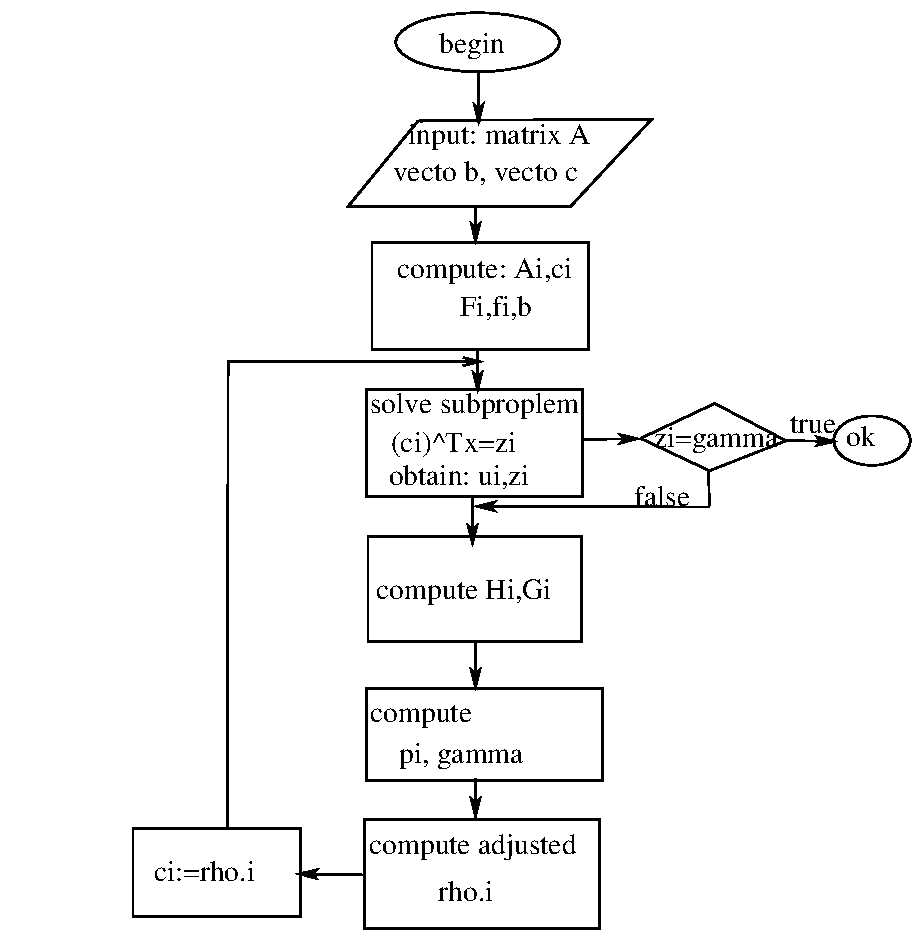
\includegraphics{sodokhoi.pdf}
\caption{sơ đồ thuật toán}\label{fig:}
\end{center}
\end{figure}

%+ 3.2.4. Triển khai xay dụng chuong trinh
\subsection{Một số thủ tục cơ bản của chương trình. }
Chương trình thể hiện phương pháp phân rã Dantzig-Wolfe có nhiều module khác nhau, được thiết kế riêng rẽ thuận tiện cho việc kiểm tra, sữa lồi, bão trì... Dưới đây là một số module cơ bản nhất:
\begin{itemize}
\item[$1.$] Private Function Doc\_m(textfile As String) As Integer 'Hàm đọc số ràng buộc từ tệp.
\item[$2.$] Private Function DocMT(textfile As String, mask As String) As String ' Hàm đọc ma trận từ tệp.
\item[$3.$] Private Function DocVT(textfile As String, mask As String) As String 'Hàm đọc vec tơ từ tệp.
\item[$4.$] Private Function phan\_ra(strA As String) As String 'Hàm phân rã ma trận A.
\item[$5.$] Private Function so\_khoi(strPR As String) As Integer 'Hàm tìm số khối xuất hiện trong ma trận A.
\item[$6.$] Private Sub GiaiBT\_DZW(textfile As String) 'Thủ tục giải bài toán D-W.
\end{itemize}

%+ Bai 3.3. Trien khai
\section{Các bước triển khai thực thi thuật toán. }
Với mục đích đưa những thuật toán có sẵn vào những ứng dụng thực tế, khóa luận này sẽ trình bày tóm tắt lại những khâu cơ bản trong quá trình triển khai thực thi một thuật toán nhằm giải quyết các bài tóan ứng dụng cụ thể. Tùy thuộc vào mục đích ứng dụng, thời gian thực hiện, chi phí, quy mô của bài toán ứng dụng, mà người ta lựa chọn những quy trình thực hiện khác nhau. Chẳng hạn dưới đây là một số bước cơ bản khi triển khai áp dụng:

\begin{itemize}
\item{\bf Bước 1. } Xây dựng mô hình định tính cho bài toán bằng cách tham biến (tham số) hoá các thành phần của bài toán thực tế. Nói cách khác là lượng hoá hoặc hình thức hoá các đối tượng thực tế bằng các ký hiệu hoặc lược đồ...Trong một số trường hợp cần phân chia, hoặc hạn chế hay rút gọn bài toán thực tế thì mới có thể mô hình hoá được dưới dạng mô hình toán học.
\item {\bf Bước 2. } Xây dựng mô hình toán học, bằng cách liên kết các đối tượng theo các mối quan hệ thành các công thức tường minh hoặc quan hệ cụ thể. Đồng thời với nó là xác định mục tiêu (một hoặc nhiều mục tiêu) cho bài toán thực tế và lượng hoá nó thành hàm mục tiêu cho bài toán tối ưu.
\item {\bf Bước 3. } Sử dụng các công cụ của toán học, cụ thể là lý thuyết tối ưu để giải quyết bài toán. Bước này cần thực hiện một cách khoa học và tuân thủ theo yêu cầu đặt ra ban đầu. Đó là phân loại bài toán, nghiên cứu các tính chất định tính, sự tồn tại nghiệm, xây dựng thuật toán giải (chương trình hoá bằng chương trình máy tính hoặc xây dựng được một lược đồ tính toán (thủ công)), đánh giá hiệu quả của phương pháp trên các phương diện: thời gian, kinh phí, phương tiện, độ chính xác, độ ổn định và tính tin cậy...
\item{\bf Bước 4. } Áp dụng vào bài toán thực tế, phân tích và kiểm định với bài toán thực tế, đánh giá kết quả và mức độ phù hợp. Có thể xảy ra hai khả năng.
\begin{enumerate}
\item Mô hình tính toán là phù hợp với thực tế. Khi đó cần tổng kết lại (thành tài liệu nghiên cứu và hướng dẫn) và có thể đưa ra áp dụng rộng rãi. Sau đó cần tính đến vấn đề kiểm định và bảo trì cũng như hướng phát triển của hệ thống trong tương lai.
\item Mô hình tính toán không phù hợp với thực tế. Khi đó cần rà soát lại các bước thực hiện để tìm ra nguyên nhân của nó. Có thể có nhiều nguyên nhân, trong đó có các nguyên nhân chủ yếu thường gặp sau: Do lựa chọn mô hình hoá toán học chưa phù hợp, công cụ giải quyết chưa phù hợp (chưa có công cụ đủ mạnh), sai số của dữ liệu (do quá trình đo đạc, quan sát, ảnh hưởng cuả môi trường...), độ chính xác và độ ổn định của thuật toán chưa được kiểm định... Do vậy cần tìm cách để khắc phục hoặc tìm hướng mới để giải lại bài toán.
\end{enumerate}
\end{itemize}
%%%%%%%%%%%%%%%%%%%%%%%%%%%%%%%%%%%%%%%%%%%
